%\section{Methodology}

\section{\acs{RTT} estimation}
\label{section:malawi:rtt}

Building on prior work presented in section \ref{section:malawi:related}, this section proposes an algorithm that scalably recovers the \ac{RTT} from one-directional traffic traces. 
% XXX: below implies microflights were used, but these aren't described (remove as appropriate)
Although \ac{RTT} estimation is a difficult problem, simplifying assumptions can be made.
For the \acs{MAWI} dataset most \acp{RTT} are relatively large, with the closest neighbouring country, South Korea, roughly 40ms away.
By only processing bidirectional traffic from Japan, the expected \ac{RTT} range can be reduced for all other traffic.
The recovery mechanism then enhances the natural periodicity of traces and scalably constructs flights associated with specific application and protocol behaviour.
In the following the mechanisms required by these two goals are described. 
%
% Why does this work?
%
In normal operation, many \ac{TCP} operations involve request-response cycles between two endpoints in which the \ac{RTT} $T$ provides a natural \emph{clock}.
Hence, the most natural way to estimate \ac{RTT} from \ac{TCP} traces is to correlate requests and responses exchanged in both directions. 
If only one direction of data is observed however, $T$ cannot be directly observed. 
Instead, it must be estimated from the way in which \ac{TCP} packets cluster in time due to the batching of request-response operations.

The \ac{TCP} \ac{cwnd} determines the number of unacknowledged bytes that a \ac{TCP} flow may maintain at any point in time. 
This can be referred to as \emph{bytes in flight} because they are in transit between the sender $S$ and the receiver $R$; an equivalent definition applies for the number of \emph{packets in flight}. 
Once $S$ has transmitted \ac{cwnd} data bytes, it will refrain from transmitting more until either some bytes are acknowledged by $R$ or \ac{cwnd} is increased by the sender. 
In the absence of losses, neither of these events can happen until a \ac{TCP} \ac{ACK} is received; this immediately reduces the number of unacknowledged bytes, but may also lead to a significant \ac{cwnd} increase (during e.g. \emph{slow start}). 
% XXX: number of unacknowledged bytes reduced, or CWND?
In the presence of losses, however, bytes can be re-sent if a packet is timed out and considered lost; in this case, the number of unacknowledged bytes is reduced.

%
% What is our main contribution, algorithmically speaking?
%
The main difficulty associated with one-sided \ac{TCP} flow reconstruction is as follows.
Let $t_1, t_2, \ldots$ be a set of times at which packets $p_1, p_2, \ldots$ were observed at $S$ en route to $R$.
Suppose that a packet $p_j$ of size $b$ is observed at time $t_j$.
In addition, suppose that approximately one \ac{RTT} $T$ later, the sender $S$ receives an \ac{ACK} $a_j$ from $R$ for the $b$ bytes of $p_j$.
At this point, the \ac{TCP} stack in $S$ will decrease the number of unacknowledged bytes by $b$, thus opening the possibility for sending additional traffic to $R$.
This can lead to another packet $p_k$ to be transmitted; let this packet be observed at time $t_k$ as it is sent towards $R$.
Assuming that processing delay is insignificant, the \ac{RTT} experienced by $p_j$ can be approximated as $T \approx t_k - t_j$.
Now consider what happens if packets are only observed in the $S \rightarrow R$ direction.
Under such conditions, it is not possible to ascertain whether $p_k$ was sent explicitly as a result of $S$ receiving the unobserved \ac{ACK} $a_j$, or whether it was sent as a result of an \ac{ACK} $a_i$ associated with a previous packet $p_i$ rather than with $p_j$.
If, however, a packet $p_l$ is eventually observed that did result from the reception of $a_j$, the \ac{RTT} can be estimated as $T \approx t_l - t_j$ with $t_l > t_k$.
Following this same reasoning, approximately one \ac{RTT} later a packet $p_m$ will be observed for which $2T \approx t_m - t_j$; this can potentially continue for as long $S$ has data to send and $R$ continues sending \acp{ACK}.
This is the underlying reason that \ac{RTT}-related periodic regularities arise when considering the timestamps of observed packets \cite{Qian:2009p429}.

The reasoning above is at the heart of the proposed algorithm to improve \ac{RTT} recovery by enhancing packet stream periodicity. 
Assume that a packet $p_j$ is observed at time $t_j$. 
Considering the set $\mathcal{T}_j$ of all values of $\Delta t = t_k - t_j$ for every $k > j$, it is apparent that it will include estimates not only for the \ac{RTT} $T$, but also for all its multiples $2T, 3T, \ldots$ 
If $t_l-t_k \approx T$ and $t_k - t_j \approx T$ then it follows that $t_l - t_j = 2T$, and this value will also be included in $\mathcal{T}_j$. 

By maintaining a set $\mathcal{T}_j$ for every packet $p_j$ observed, at least some of its values will correspond to estimations of multiples of the \ac{RTT}. 
It then follows that by creating a set $\mathcal{T}$ that includes values calculated starting from every packet $p_j$ so that $\mathcal{T} = \cup_j \mathcal{T}_j$, numerous estimates for $2T, 3T, \ldots$ will also be included. 
Hence, the probability density function $H(t)$ of the values in $\mathcal{T}$ should show peaks around multiples of the \ac{RTT} (see Figure \ref{fig:histogram}). 

\begin{figure}
  \centering
  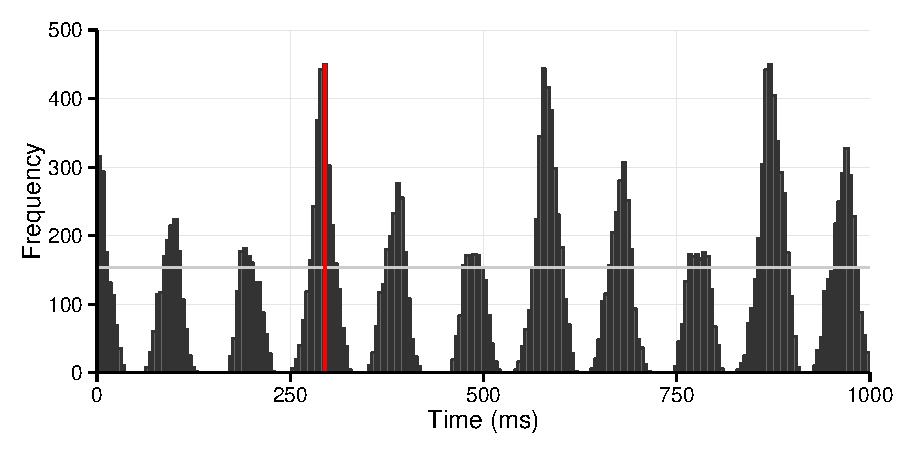
\includegraphics[width=0.8\textwidth]{figures/malawi/rttbin.pdf}
  \caption[$H(t)$ for flow displayed in figure \ref{fig:hostlimited}.]{$H(t)$ for flow displayed in figure \ref{fig:hostlimited}. The horizontal line delimits $\overline{H}$ while the highlighted bin denotes the bidirectional \acp{RTT} estimate.\label{fig:histogram}}
\end{figure}

%
% Explain why did we use FFT
%
The algorithmic recovery of $T$ from $H(t)$ presents additional challenges. 
In particular, $H(t)$ may include a large number of \ac{RTT} multiples, and a peak will be found for all of them. 
Crucially, all these peaks may be of comparable magnitude, complicating the task of selecting a single peak.
Moreover, these peaks need not be very pronounced, with histogram bins in close proximity of the peaks have very similar values as the peak itself. 
As such, taking \ac{RTT} candidates directly from $H(t)$ may result in a large set of similarly-valued bins situated around a peaks at multiples of the \ac{RTT}. 

Three recovery algorithms for $T$ are attempted.
First, as a baseline, the highest peak in $H(t)$ is selected as a candidate for $T$. 
In addition, expanding upon the work of Qian et al.\ \cite{Qian:2009p429} a frequency-domain representation of $H(t)$ is used to identify $T$. 
This is done by selecting the highest peak of $|\hat{H}(\omega)|^2$, the \emph{energy spectral density} of $H(t)$ (i.e. the norm squared of the Fourier transform of $H(t)$). 
Finally, a custom utility-based technique that operates directly on $H(t)$ is proposed which achieves superior performance to both of the aforementioned methods.

%\subsubsection{FFT-Based RTT Recovery}
%We extract periodicity information from $H(t)$ by looking at $\hat{H}(\omega)$, the \emph{energy spectral density} of $H(t)$. Formally, $\hat{H}(\omega)$ is defined as the norm squared of the Fourier transform of $H(t)$, so that $\hat{H}(\omega) = |\mathcal{F}(H(t))|^2$. Using $\hat{H}(\omega)$ markedly improves the quality of our RTT estimation because the frequency peak corresponding to the RTT usually accounts for a much larger proportion of the total frequency domain energy than other peaks in $\hat{H}(\omega)$, leading to a much simpler discrimination of the true RTT. However, due to RTT changing during the lifetime of a flow, and also due to the expected noise associated with real-life data sources, $\hat{H}(\omega)$ can also occasionally include large peaks at frequencies unrelated to the RTT. In order to filter these out, we take a set of 10 frequency candidates from $\hat{H}(\omega)$, and use their associated periods as RTT candidates in our flow reconstruction algorithm (see Section \ref{
%subsection:malawi:flightAggregation}). We then select that RTT candidate which exhibits the smallest error, that is, that one which yields closest agreement with observed data.

%
% Algorithmic hacks
%
%To streamline our algorithm for streaming use, we use the following heuristics and approximations. Firstly, we define a range $[T_{\min}, T_{\max}]$ representing the range over which we find the RTT values of interest. Then, for each packet $p_j$, we build a subset $\mathcal{T}_j'$ of $\mathcal{T}_j$ by including all values of $t_j - t_k < T_{\max}$. We then generate $\mathcal{T}' = \cup_j \mathcal{T}_j'$ and approximate $H(t)$ by considering a histogram of the values in $\mathcal{T}'$. As usual, we do this by counting the frequency with which its values are observed in the ranges $[0,\tau)$, $[\tau, 2\tau)$, $[2\tau, 3\tau), \ldots$ where $\tau$ is the time resolution required. 


\subsection{Utility-Based \acs{RTT} Recovery}
\label{sect:utilityBasedRecovery}

This method relies not on the identification of periodicities, but on explicitly matching experimentally found signatures. 
To this end, we consider the peaks of $H(t)$, which are then considered \ac{RTT} candidates.  
However, trivial discriminators (such as simply selecting the highest peak) are not reliable. 
In this case, it was found experimentally that repeatable peaks and troughs also occur at multiples and sub-multiples of $T$, with the most important ones being $\frac{T}{3}$, $\frac{T}{2}$, $T$ and $2T$. 
We design this detection algorithm around the idea that a given pattern of peaks and troughs can identify $T$.

If we define $\overline{H}$ as the mean height of $H(t)$, we can define a per-peak utility function $p(t)$ so that 
\begin{equation*}
p(t) = 1.0 - \exp\left(-2.0 \left(\frac{H(t)}{\overline{H}}\right)\right) \mbox{.}
\end{equation*}
This function has several advantageous properties: it is 0 if $H(t)$ is zero, 1 if $H(t)$ is infinite, and $0.5$ if $H(t) = \overline{H}$.  
In other words it is a measure of the \emph{peakiness} of the data, with $p=1$ identifying an infinitely high peak, $p=0$ identifying an empty histogram bin (trough), and $p=\frac{1}{2}$ implying that $H(t)$ is of exactly average height at that point. 
We can then score each candidate using the following utility function:
$$
P(t) = 1.5 p(t) + p(2t) - p\left(\frac{t}{2}\right) - p\left(\frac{t}{3}\right).
$$
That is, the candidate \ac{RTT} $t$ scores highly if it is itself a peak, if it has a peak at a multiple $2t$, and if it also manifests troughs at sub multiples $\frac{T}{2}$ and $\frac{T}{3}$.
The factor of 1.5 was added after observations showed that the peak at $T$ was the most important factor in determining whether a candidate was the true \ac{RTT}. 
Similarly, additional multiples and sub multiples were excluded as they showed very limited discriminating power experimentally.

\begin{figure}
  \centering
  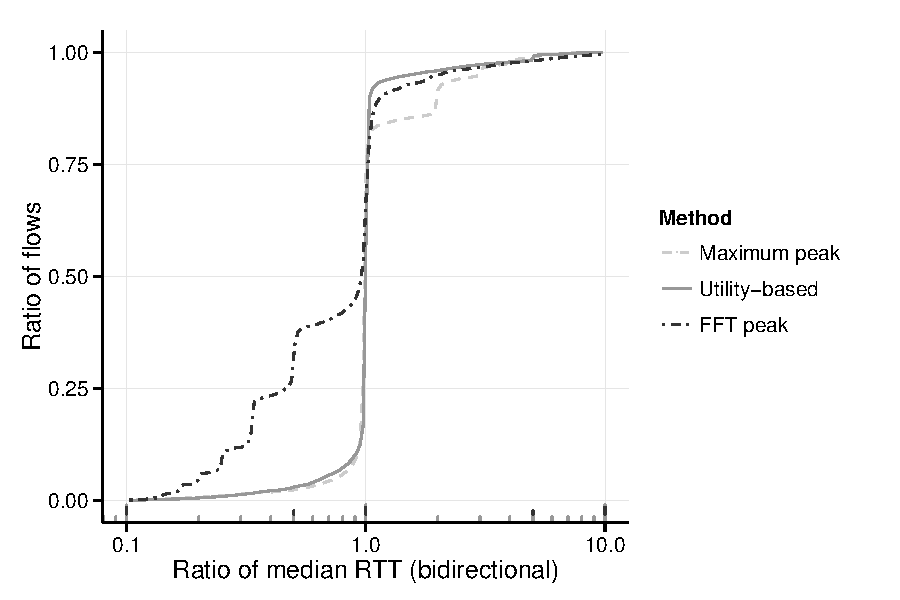
\includegraphics[width=0.8\textwidth]{figures/malawi/rttcomp.pdf}
  \caption{Accuracy of \ac{RTT} estimator when compared to the median value of bidirectional estimate.}
\end{figure}

\subsection{Comparing recovery algorithms}
\label{sect:comparingRecoveryAlgos}
As described in Section \ref{subsection:malawi:PeriodicEnhancement}, $H(t)$ is calculated in such a way that \ac{RTT} periodicity is amplified. 
This means that \acs{FFT}-based techniques could potentially perform better on $H(t)$ than on the packet stream with no pre-processing. 
However, this is complicated not only because $H(t)$ contains periodicities at multiples of $T$, but also discontinuities that generate harmonics at frequency multiples of the \ac{RTT} fundamental. 
Hence, although the \acs{FFT} $|\hat{H}(\omega)|$ of $H(t)$ is much cleaner than that of the packet inter arrival time series on its own, its maximum peak rarely coincides exactly with the \ac{RTT} clock (this corroborates reports by Qian et al.\ \cite{Qian:2009p429}). 
Thus, applying the \acs{FFT} leads to another \emph{peak detection problem} in which the \ac{RTT} fundamental needs to be extricated from its harmonics and sub-harmonics. 
The trivial solution to this problem, the application of a bandpass filter around the \ac{RTT} frequency, is of course infeasible because the bandwidth and 
centring of such a filter depend on the \ac{RTT} which is itself unknown.
The utility-based algorithm described in Section \ref{sect:utilityBasedRecovery} can hence be applied in either the time domain or the frequency domain; we chose to do it on the former on the interest of expediency and lower computational cost.

\newcommand{\RTTHeader}{Below & Above}
\newcommand{\SmallFlowName}{\textless 10MB}
\newcommand{\LargeFlowName}{\textgreater 10MB} 
\begin{table}\footnotesize\centering
\begin{tabular}{  
@{}
$>{\raggedleft\arraybackslash}p{2.5cm}@{\hskip 1.0cm}
^r
^r@{\hskip 0.5cm}
^r
^r
@{}
}
\toprule
\rowstyle{\scshape\bfseries}
\multirow{2}{*}{\parbox[][0.7cm][b]{2.5cm}{Sample data}} & 
\multicolumn{2}{c}{\scshape\bfseries{Peak (\%)}} &
\multicolumn{2}{c}{\scshape\bfseries{Utility (\%)}} \\
\cmidrule(r{0.5cm}){2-3}\cmidrule{4-5}
\addlinespace[-0.6em] \rowstyle{\scriptsize\scshape}
& Below & Above & Below & Above \\
\midrule


\raggedright\scshape\arraybackslash Receiver side \\
%\multicolumn{1}{l}{\scshape Receiver side}\\
$flow < 10$MB & 4.31 & 9.13 && 4.58 & 6.35
\\ 
$flow > 10$MB & 6.72 & 6.43 & 4.97 & 5.33
\\ 
\addlinespace[0.6em]
\raggedright\scshape\arraybackslash Sender side \\
$flow < 10$MB & 2.94 & 8.37 && 3.29 & 4.80
\\ 
$flow > 10$MB & 6.41 & 9.06 & 5.40 & 11.06
\\ 
\bottomrule
\end{tabular}
\caption[Performance of \acs{RTT} recovery algorithms]
{\label{table:rttRecovery}Performance of peak-based and utility-based \acs{RTT} recovery algorithms, showing proportion of flows for each sample dataset with estimates below and above bidirectional estimate.}
\vspace{-3mm}
\end{table}

The performance of the analysed \ac{RTT} recovery mechanisms is presented in Table \ref{table:rttRecovery}, that shows the percentage of total flows below and above the \ac{RTT} range given by the bidirectional estimates.
We separate things for \emph{inbound} traffic (where we are positioned at the receiver side) and \emph{outbound} traffic (where we are positioned at the sender side). 
The utility-based algorithm is particularly useful to address \ac{RTT} underestimation for flows over 10MB in size, which is our main objective since precisely that kind of estimation error would interfere with our ability to correctly decouple application behaviour from \ac{RTT}-scale dynamics.


%For the most part, the utility based method improves on underestimation, which is our main objective since that would interfere with our flight reconstruction (i.e. generate lots of gaps).
%The exception (kind of) is traffic from the sender side, which in our training set (one week per year), had quite a lot of host limited traffic (paced out, no signal to recover).
%In this case, not a problem, since if the flow is long enough multiples of the RTT will still reveal host limitation, but will give us a smaller window..

